\chapter{Basic Definitions}

In this chapter basic definitions necessary in the following chapters are placed. This definitions are cited from \cite{RepAndConsistentAnswer, QueryXML, ImprovingXML}.


\section{XML Trees and DTDs}
\begin{define}[Tree]
Given an alphabet of nodes $\mathbb{N}$ and an alphabet of node labels $\Sigma$, a {\sl tree} $T$ over $\mathbb{N}$ and $\Sigma$ is a tuple $(r_T, N_T, E_T, \lambda_T)$, where $N_T \subseteq \mathbb{N}$ is the set of nodes, $\lambda_T : N_T \to \Sigma$ is a node labelling function, $r_T \in N_T$ is the distinguished root of $T$, and $E_T \subseteq N_T \times N_T$ is an set of edges such that starting from any node $n_i \in N_T$ it is possible to reach any other node $n_j \in N_T$, walking through a sequence of edges $e_1,\dots,e_k$ which are connected and acyclic.
\end{define}

\noindent Let also denote the set of leaf nodes as $Leaves(T)$ and the set of trees defined over an alphabet of node labels $\Sigma$ as $T_\Sigma$.

\begin{define}[XML Tree]
{\sl XML tree} is a pair $XT=\langle T,\delta \rangle$, where:
	\begin{enumerate}
		\item $T = (r, N, E, \lambda)$ is a tree in $T_{\tau\cup\alpha\cup\{S\}}$, where $\tau$ is a tag alphabet, $\alpha$ is an attribute name alphabet and $S$ is a symbol not belonging to $\tau\cup\alpha$ (representing \texttt{\#PCDATA} content of elements)$;$
		\item given a node $n$ of $T$, $\lambda(n) \in \alpha \cup \{S\} \Leftrightarrow n \in Leaves(T);$
		\item $\delta : Leaves(T) \rightarrow Str$, where $Str$ is a string alphabet, is a function associating a (string) value to every leaf of $T$.
	\end{enumerate}\qed
\end{define}

\begin{example}
\end{example}

\begin{figure}
    \centering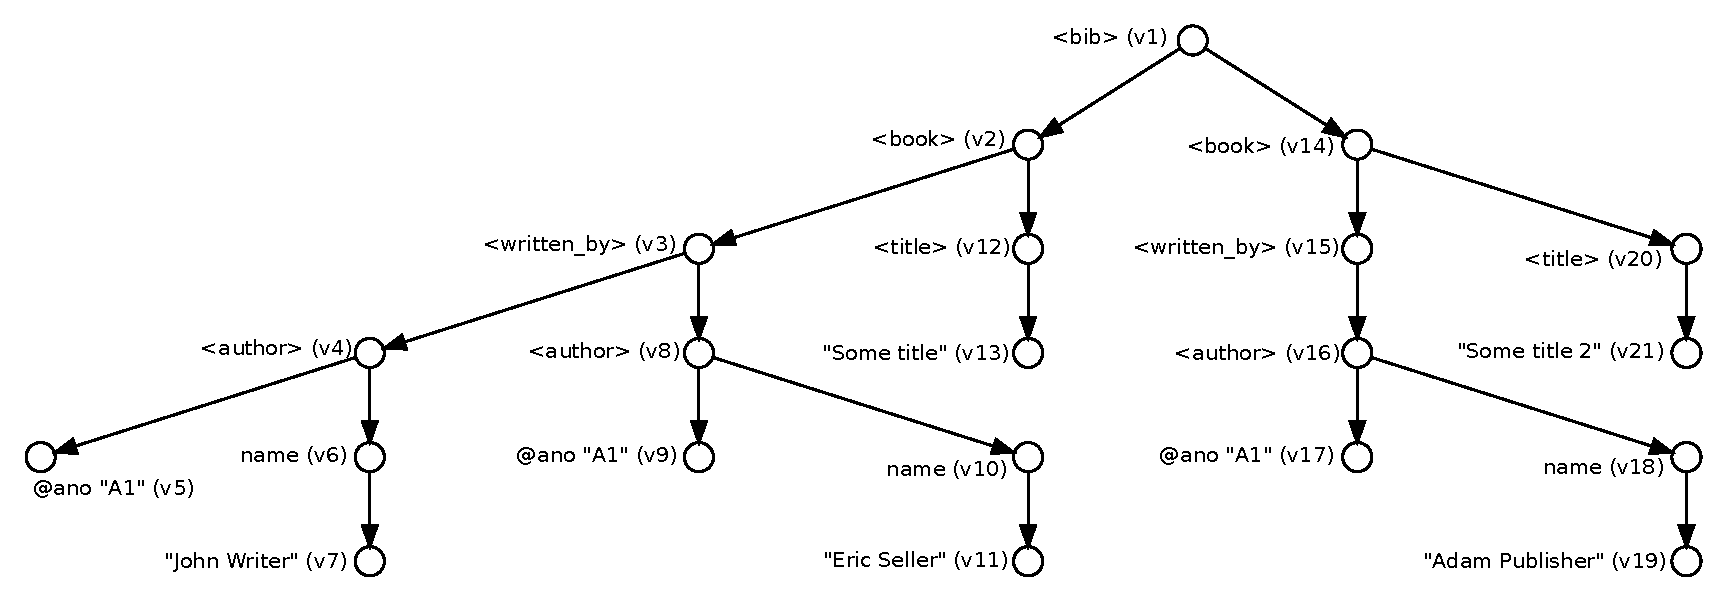
\includegraphics[scale=\myscale]{example1-new}
	\caption{XML Tree} \label{example1}
\end{figure}

\begin{define}[DTD]\label{dtdDef}
{\sl DTD} is a tuple $D = (\tau, \alpha, P, R, rt)$ where: i) $\tau$ and $\alpha$ are of the same definition as in the \emph{XML tree}; ii) $P$ is the set of \emph{element type definitions}; iii) R is the set of \emph{attribute lists}; iv) $rt \in \tau$ is the tag of the document root element.\qed
\end{define}

\begin{define}[Path]
{\sl Path} p on a DTD $D = (\tau, \alpha, P, R, rt)$ is a sequence $p = s_1, \dots, s_m$ of symbols in $\tau \cup \alpha \cup \{S\}$ such that:
	\begin{enumerate}
		\item $s_1=rt$;
		\item for each $i$ in $2..m-1$, $s_i \in \tau$ and $s_i$ appears in the element type definition of $s_{i-1}$;
		\item $s_m \in \alpha \rightarrow s_m$ appears in the attribute list of $s_{m-1}$;
		\item $s_m \in \tau \cup \{S\} \rightarrow s_m$ appears the element type definition on $s_{m-1}$.
	\end{enumerate}\qed
\end{define}

As we defined \emph{path} on a DTD $D$, let denote as $paths(D)$ the set of paths which can be defined on a DTD $D$. Also another important notion is $p(XT)$ (or $\{[\![p]\!]\}$), which is the set of nodes from XML tree $XT$ conforming DTD $D$, which can be reached by the path $p \in paths(D)$, starting from the root of $XT$. The set of nodes reachable from a node $v$ following path $p$ is denoted as $\{v[\![p]\!]\}$. When there is only one node in $\{v[\![p]\!]\}$, we use $v[\![p]\!]$ to denote this node. Moreover, let denote $XT.p$ the \emph{answer} of the path $p$ applied on $XT$ , that is:
\begin{itemize}
	\item[-] if $p \in EPath(D)$, where $EPath(D)$ denotes the set of the paths whose last symbol denotes an element, then $XT.p = p(XT)$
	\item[-] if $p \in StrPath(D)$, where $StrPath(D)$ denotes the set of paths whose last symbol denotes either the textual content of an element or an
attribute, then $XT.p = \{\delta_T(x)|x \in p(XT)\}$.
\end{itemize}

\section{Integrity Constraints and Functional Dependencies}

In relational database $D$, correspondence between values $A$ and $B$ in the tuple of $D$, models the functional dependency denoted as $A \rightarrow B$. Because in XML is not such a standard tuple concept, authors introduce the concept of tree tuples, corresponding to relational databases concept of tuples.

\begin{define}[Tree Tuple]
Given an XML tree XT conforming the DTD D, a tree tuple t of XT is a maximal sub-tree of XT such that, for every path $p \in paths(D)$, t.p contains at most one element.\qed
\end{define}

\begin{define}[Functional Dependency]
Given a DTD D, a functional dependency on D is an expression of the form $S \rightarrow p$, where S is a finite non empty subset of $paths(D)$ and p is an element of $paths(D)$.\qed
\end{define}

Given an XML tree $XT$ conforming a DTD $D$ and a functional dependency $F : S_1 \rightarrow S_2$ , we say that $XT$ satisfies $F (XT \models F )$ if for each pair of tree tuples $t_1, t_2$ of $XT$, $t_1.S_1 = t_2.S_1 \land t_1.S_1 = \emptyset \Rightarrow t_1.S_2 = t_2.S_2$ . Given a set of functional dependencies $\mathcal{FD} = \{F_1 , \dots, F_n\}$ over $D$, we say that $XT$ satisfies $\cal FD$ if it satisfies $F_i$ for every $i \in 1..n$.

\todo[inline]{tuto treba doplnit definiciu satisfiability of tree to FD}
\begin{define}[satisf tree to FD]\label{treeSatisf}
\end{define}

\todo[inline]{tuto treba doplnit definiciu integrity constraints}
\begin{define}[Integrity Constraints]\label{integConstr}
\end{define}
